% simulation_text.tex

\documentclass[12pt]{article}
\usepackage{setspace}
\usepackage{graphicx}
\usepackage{amsmath}
\usepackage{natbib} %for citet and citep
\usepackage{syntonly}
\usepackage{esdiff} %for writing partial derivatives
\usepackage{url} %for inserting urls
\usepackage{placeins}
\usepackage{natbib}
% \usepackage{comment} %for excluding figures
% \excludecomment{figure} % for printing without figures
% \syntaxonly % for quickly checking document
%set document settings

% \doublespacing % from package setspacs

% table font size
\let\oldtabular\tabular
\renewcommand{\tabular}{\scriptsize\oldtabular}

\title{Appendix: Oil Prices and Field Production: A Montecarlo Simulation Experiment}
\author{Johannes Mauritzen\\
		Department of Business and Management Science\\
        NHH Norwegian School of Economics\\
        Helleveien 30, 5045\\
        Bergen, Norway\\
        johannes.mauritzen@nhh.no\\
        \url{jmaurit.github.io}\\
		}
\date{\today}


\begin{document}
% \begin{spacing}{1} %sets spacing to single for title page
	\maketitle


\section{Introduction}

The data set used in this paper has a complex structure.  The dependent variable - field level oil production - has a non-linear autocorrelated structure.  The production profiles are also correlated with each other - leading to a bell-shaped total production curve.  In addition the exogenous variable of interest - oil prices - are autocorrelated and non-stationary.    In such a setting, standard rules for inference may not hold. 

In this appendix I instead present a Monte Carlo simulation experiment.  Generating artificial data that is similar in character to the data used, I first show how failing to properly control for the production profile can lead to a biased estimation of the effect of oil prices.  I then show how using a generalized additive model can lead to better estimates.  

I use the R statistical programming language \citet{r_core_team_r:_2013} for the analysis.  For illustration, I include code snippets in this document.  The full code for the analysis can be found at \url{jmaurit.github.io\#oil_prices}. The figures shown are created using the r package ggplot2 \citet{wickham_ggplot2:_2009}.

\section{Generating Data} 

The first step is generate a set of fields from a size distribution.  In the simulation, I generate 77 fields from a exponential normal distribution with mean 2.3 and standard deviation of 1.5.  This is similar to the distribution of the actual 77 productive Norwegian fields. 
\begin{verbatim}
field_size<-round(exp(rnorm(77, mean=2.3, sd=1.5)), digits=1)
\end{verbatim}

Using the generated field sizes as an input, I then create a function to generate starting times.  The goal here is to mimic what is called creaming in the exploration industry - the tendency of finding and starting production on larger fields first. For fields that are smaller than 10 million SM3, I generate a starting time from a uniform distribution with endpoints 1975 and 2008.  For larger fields, I generate a starting time from a normal distribution with standard deviation of 10 and a mean as in formula 1:

\begin{equation}
mean_start(size) = trunc(1973 + (max + 300)/size)
\end{equation}

\begin{verbatim}
gen_year<-function(size, maxsize){
	#let small fields be distributed uniformly from 1975 to 2013
	if(size<10){
		year<-trunc(runif(1, 1975, 2008))	
	} else{	#while large fields should be more common earlier on
		range<-FALSE
		while(range==FALSE){
			year<-trunc(rnorm(1,mean=(1973+(maxsize+300)/(size+300)), sd=10))
			ifelse(year>=1970 & year<=2013, range<-TRUE, range<-FALSE)
			}	
		}
return(year)	
}
\end{verbatim}

Generating the starting times in this way was essentially ad-hoc.  However the method is sufficient since the purpose of this exercise is not to model the underlying physical and economic processes, but rather to generate data that shares key similarities with the actual data.

In the simulation I use the actual Brent oil price series shown in figure \ref{oil_price_series}.  This series can be shown to be non-stationary.  In order to get reliable inference in a simpler time-series setting the solution might be to take the first difference of the series.  This is not possible in this setting since it is the actual levels of oil prices that are important.  Intuitively, identification comes from comparison of fields of similar size and at similar points in their production lifetime but at periods at differing oil prices.  This variation would be discarded by purely looking at first differences.

\begin{figure}
	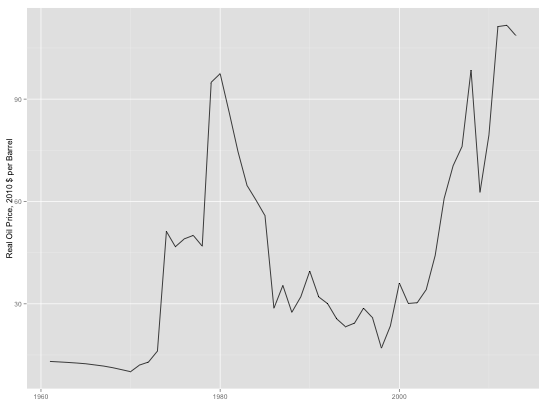
\includegraphics[width=1\textwidth]{figures/oil_price_series.png}
	\caption{The Real Price of Brent Traded Oil from 1960 to 2013 in 2010 U.S. Dollars.}
	\label{oil_price_series}	
\end{figure}

So far, all the simulated data has been outside the Monte Carlo function.  The data is treated as being fixed.Within the Monte-Carlo loop I create a function that takes as input a fields size, start date as well as the price series and generates a production profile.  The code for this function is below.  

\begin{verbatim}
gen_production<-function(field, prices){
	size<-field[1]
	start<-field[2]
	name<-field[3]

	names(prices)<-c("year", "price")
	t<-trunc(sqrt(size)) + 3  #generate production time
	prod_time<- -t:(t)
	year=start:(start+2*t-1)

	#use a cumulative logistic function to represent shape of function
	cum_production = 1/(1+exp(-(prod_time)/3))*size

	#take difference to create production per year
	prod_shape = diff(cum_production)
	production<-data.frame(year, prod_shape)
	
	#Formula: log(production) = f`(time) + beta*log(price) + epsilon
	
	production$prod<-production$prod_shape*
	exp(beta0*production$price*rlnorm(length(production$price), meanlog=0, sdlog=.05))

	return(production)
}
\end{verbatim}

First, the production time of the field is created as a deterministic function of field size.  I then model cumulative production from the field over time as a logistic function as in equation \ref{cumProd_equation}.  This series is then first-differenced to create the general production profile.  

\begin{equation}
% 1/(1+exp(-(prod_time)/3))*size
cumProd=\frac{size}{1+exp(\frac{-prodTime_t}{3})}
\label{cumProd_equation}

\end{equation}

I multiply the production profile series with an exponential price term and a coefficient representing the effect of price as well as a random component with mean 0 and standard deviation .05 drawn from a log-normal distribution.  Taking the logarithm of both sides, the production series for a given field can be written as equation \ref{production_equation}.  Importantly, the term $\beta$ represents the true effect of price on production.  

\begin{equation}
log(production_t)=log(prodShape_t) + \beta price_t + \epsilon_t
\label{production_equation}
\end{equation}

Within the Monte-Carlo loop, production data for each field is generated as above.  Thus the variation in each run of the Monte Carlo simulation is the random term $\epsilon_t$ from equation \ref{production_equation}. 

An example of the data generated can be seen in figure \ref{simulated_production}.  By inspection, it appears reasonably similar to the data on actual oil production on the Norwegian Continental Shelf.  

\begin{figure}
	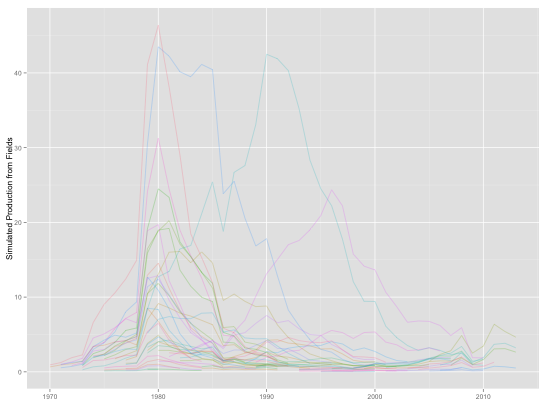
\includegraphics[width=1\textwidth]{figures/simulated_production.png}
	\caption{Simulated production of 77 oil fields}
	\label{simulated_production}	
\end{figure}


\section{Estimation of Coefficient}

Within the Monte Carlo function, a regression is run using the gam() function from the package mgcv \citet{wood_generalized_2006}.  This will handle both estimation of linear models or generalized additive models, depending on what formula is passed to the Monte Carlo function.  

\begin{verbatim}
gam_sim<-gam(formula,
	family=gaussian(link=log), weights=size, data=sim_fields)
summary(gam_sim)
\end{verbatim}

Outside of the Monte Carlo function, First I specify a linear regression formula with a 3rd degree polynomial terms to control for the production profile as below.  

\begin{verbatim}
formula_0=formula(prod~time_to_peak + time_to_peak_sq + time_to_peak_cu + 
	peak_to_end + peak_to_end_sq + peak_to_end_cu +size + price)
\end{verbatim}

I then replicate the data 1000 times, letting the $\beta$ term equal zero, that is having no effect of prices on oil production.  The formula used is shown below, where $gam_mc()$ is the Monte Carlo function.  

\begin{verbatim}
gamm_mc_0<-replicate(1000, gam_mc(beta=0, formula=formula_0, use_true_prices=TRUE))
\end{verbatim}

The above line returns 1000 estimates of $\beta$ from the linear regression specification.  Figure \ref{lin_model_price_mc} shows the results in the form of a histogram.

\begin{figure}
	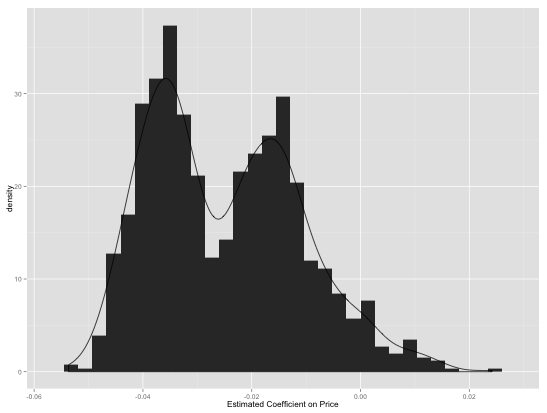
\includegraphics[width=1\textwidth]{figures/lin_model_price_mc.png}
	\caption{Estimated coefficients on price from linear model from Monte Carlo Experiment}
	\label{lin_model_price_mc}	
\end{figure}

As the figure shows, a negative bias in the coefficient is apparent.  The distribution appears double-peaked, with most of the estimates of $\beta$ begin between -.05 and -.01.   

Now consider a specification using a smooth term for the production profile as below.

\begin{verbatim}
formula_1= formula(prod~s(prod_time,size) + price)
\end{verbatim}

Now, the production profile is modeled as a smooth function of production time and size with an additive linear term for price.  Unlike the specification in the body of the article, I do not specify separate smooth terms for pre- and post-peak.  This is simply because I know that the logistic function I used to create the shape of the production profile is symmetric.  

The results of running the Monte Carlo experiment with the specification with the smoothed term are shown in figure \ref{gam_model_price_mc.png}.  Here the estimated coefficient on the price term is centered close to zero, correctly reflecting the true $\beta$.

\begin{figure}
	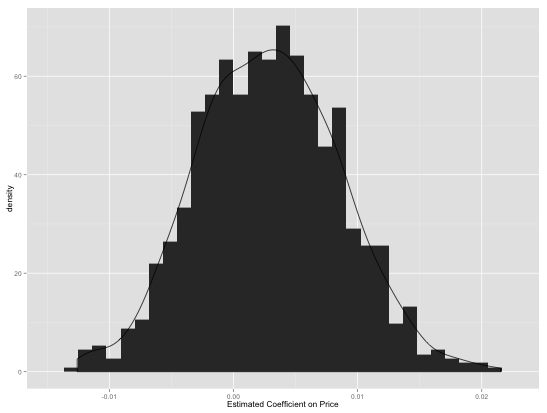
\includegraphics[width=1\textwidth]{figures/gam_model_price_mc.png}
	\caption{Estimated coefficients on price from GAM model from Monte Carlo Experiment}
	\label{gam_model_price_mc.png}	
\end{figure}

\FloatBarrier

\bibliographystyle{plainnat}
\bibliography{oil_prices}


\end{document}